\documentclass{article}

% content/resources/templates/preamble.tex
\usepackage[margin=0.6in]{geometry}
\author{Milav Dabgar}
\usepackage{amsmath,amssymb,amsthm}
\usepackage{booktabs}
\usepackage{multirow}
\usepackage{xcolor}
\usepackage{tcolorbox}
\tcbuselibrary{breakable,skins}
\usepackage[colorlinks=true,linkcolor=blue]{hyperref}
\usepackage{titlesec}
\usepackage{enumitem}
\usepackage{tikz}
\usepackage{pgfplots}
\usepackage{circuitikz}
\usepackage[version=4]{mhchem}
\usepackage{longtable}
\usepackage{array}
\usepackage{float}
\usepackage{caption}
\usepackage{listings}

\lstset{
  basicstyle=\small\ttfamily,
  breaklines=true,
  breakatwhitespace=false,
  postbreak=\mbox{\textcolor{red}{$\hookrightarrow$}\space},
  float=false,
  numbers=left,
  numberstyle=\tiny\color{gray},
  numbersep=10pt,
  xleftmargin=2em,
  keywordstyle=\color{blue},
  commentstyle=\color{green!60!black},
  stringstyle=\color{purple},
  backgroundcolor=\color{gray!5},
  showstringspaces=false,
  tabsize=2,
  captionpos=b,
  keepspaces=true,
  columns=flexible
}

\pgfplotsset{compat=1.18}
\usetikzlibrary{shapes,arrows,positioning,calc,patterns,decorations.pathmorphing,decorations.markings,arrows.meta}

% Color scheme
\definecolor{headcolor}{RGB}{0,102,204}
\definecolor{keycolor}{RGB}{220,20,60}
\definecolor{solutioncolor}{RGB}{34,139,34}
\definecolor{mnemoniccolor}{RGB}{148,0,211}
\definecolor{codecolor}{RGB}{0,0,100}

% Spacing
\setlength{\parskip}{3pt}
\setlist[itemize]{nosep}
\setlist[enumerate]{nosep}

% Title formatting
\titleformat{\section}{\Large\bfseries\color{headcolor}}{\thesection}{1em}{}
\titleformat{\subsection}{\large\bfseries\color{headcolor}}{\thesubsection}{1em}{}

% Pandoc tightlist compatibility
\providecommand{\tightlist}{%
  \setlength{\itemsep}{0pt}\setlength{\parskip}{0pt}}

% Pandoc longtable compatibility
\newcounter{none}
\def\thenone{}


% content/resources/templates/english-boxes.tex

% Custom environments
\newtcolorbox{solutionbox}{
 breakable,
 enhanced,
 colback=solutioncolor!5!white,
 colframe=solutioncolor!75!black,
 fonttitle=\bfseries,
 title=Solution
}

\newtcolorbox{solutionboxnobreak}{
 colback=solutioncolor!5!white,
 colframe=solutioncolor!75!black,
 fonttitle=\bfseries,
 title=Solution
}

\newtcolorbox{keyformula}{
 breakable,
 enhanced,
 colback=keycolor!5!white,
 colframe=keycolor!75!black,
 fonttitle=\bfseries,
 title=Key Formula
}

\newtcolorbox{mnemonicboxenv}{
 breakable,
 enhanced,
 colback=mnemoniccolor!5!white,
 colframe=mnemoniccolor!75!black,
 fonttitle=\bfseries,
 title=Mnemonic
}

\newcommand{\mnemonicbox}[1]{%
  \begin{mnemonicboxenv}
    #1
  \end{mnemonicboxenv}
}


% Custom commands for GTU solutions
% This file defines semantic commands for consistent formatting

% Question command with automatic formatting
\newcommand{\question}[2]{%
  \section*{Question #1}%
  \textbf{#2}%
}

% OR question variant
\newcommand{\questionor}[2]{%
  \section*{Question #1 OR}%
  \textbf{#2}%
}

% Proper table environment with caption
\newenvironment{answertable}[1]{%
  \begin{table}[htbp]
  \centering
  \caption{#1}
}{%
  \end{table}
}

% Proper figure environment for diagrams
\newenvironment{answerdiagram}[1]{%
  \begin{figure}[htbp]
  \centering
  \caption{#1}
}{%
  \end{figure}
}

% Semantic markup for key terms
\newcommand{\keyword}[1]{\textbf{#1}}
\newcommand{\code}[1]{\texttt{#1}}
\newcommand{\classname}[1]{\texttt{#1}}
\newcommand{\methodname}[1]{\texttt{#1}}

% Proper quotation marks
\newcommand{\mnemonic}[1]{``#1''}


\title{Elements of Electrical \& Electronics Engineering (1313202) - Summer 2024 Solution}
\date{June 13, 2024}

\begin{document}
\maketitle

\questionmarks{1(a)}{3}{Define: 1. Node, 2. Loop, 3. Branch}

\begin{solutionbox}
\begin{enumerate}
    \item \textbf{Node:} A point in a circuit where two or more circuit elements meet or connect.
    \item \textbf{Loop:} A closed path in a circuit that starts and ends at the same point without passing through any node more than once.
    \item \textbf{Branch:} A path or element connecting two nodes in a circuit.
\end{enumerate}
\end{solutionbox}

\begin{mnemonicbox}
\mnemonic{Never Loop Between: Nodes Link, Loops Bound, Branches Establish connections}
\end{mnemonicbox}

\questionmarks{1(b)}{4}{Write statement of Superposition theorem and Maximum power transfer theorem.}

\begin{solutionbox}
\begin{itemize}
    \item \textbf{Superposition Theorem:} In a linear circuit with multiple sources, the response (voltage or current) in any element equals the algebraic sum of responses caused by each source acting alone, with all other sources replaced by their internal impedances.
    \item \textbf{Maximum Power Transfer Theorem:} Maximum power is transferred from source to load when the load resistance equals the source's internal resistance ($R_L = R_S$).
\end{itemize}

\begin{center}
\begin{tikzpicture}[node distance=2cm, auto]
    % Superposition
    \node [gtu block] (src) {Sources};
    \node [gtu block, right=of src] (ind) {Individual\\Responses};
    \node [gtu block, right=of ind] (sum) {Sum = Total\\Response};
    
    \draw [gtu arrow] (src) -- (ind);
    \draw [gtu arrow] (ind) -- (sum);
    
    % Max Power
    \node [gtu block, below=1.5cm of src] (source) {Source $R_S$};
    \node [gtu block, right=of source] (load) {Load $R_L$};
    \node [gtu block, right=of load] (cond) {Max Power\\when $R_S = R_L$};
    
    \draw [gtu dashed arrow] (source) -- (load);
    \draw [gtu arrow] (load) -- (cond);
\end{tikzpicture}
\captionof{figure}{Concepts of Superposition and Max Power Transfer}
\end{center}
\end{solutionbox}

\begin{mnemonicbox}
\mnemonic{Sum Powers Matched: Sum individual powers; Match resistance for maximum}
\end{mnemonicbox}

\questionmarks{1(c)}{7}{Explain Kirchhoff's Voltage Law and Kirchhoff's current Law.}

\begin{solutionbox}
\begin{tabulary}{\linewidth}{|L|L|L|}
\hline
\textbf{Law} & \textbf{Explanation} & \textbf{Mathematical Form} \\ \hline
\textbf{Kirchhoff's Voltage Law (KVL)} & The algebraic sum of all voltages around any closed loop in a circuit equals zero. & $\sum V = 0$ \\ \hline
\textbf{Kirchhoff's Current Law (KCL)} & The algebraic sum of all currents entering and leaving a node equals zero. & $\sum I = 0$ \\ \hline
\end{tabulary}

\begin{center}
\begin{tabular}{cc}
\begin{circuitikz}[scale=0.8]
    \draw (0,0) to[battery1, l=$V_1$] (0,3) -- (3,3) to[R, l=$V_2$] (3,0) -- (0,0);
    \draw (1.5,1.5) node[circle, draw] {Loop};
    \node at (1.5,-0.5) {KVL: $V_1 - V_2 = 0$};
\end{circuitikz}
&
\begin{circuitikz}[scale=0.8]
    \draw (0,0) node[circle,fill,inner sep=2pt,label=above:Node] (N) {};
    \draw[<-] (N) -- (-1.5, 1) node[left] {$I_1$};
    \draw[<-] (N) -- (-1.5, -1) node[left] {$I_2$};
    \draw[->] (N) -- (1.5, 1) node[right] {$I_3$};
    \draw[->] (N) -- (1.5, -1) node[right] {$I_4$};
    \node at (0,-1.5) {KCL: $I_1 + I_2 = I_3 + I_4$};
\end{circuitikz}
\end{tabular}
\captionof{figure}{KVL and KCL Diagrams}
\end{center}

\begin{itemize}
    \item \textbf{Physical interpretation of KVL:} Energy is conserved in a circuit loop.
    \item \textbf{Physical interpretation of KCL:} Charge is conserved at circuit nodes.
    \item \textbf{Application of KVL:} Finding unknown voltages in circuit loops.
    \item \textbf{Application of KCL:} Finding unknown currents at circuit junctions.
\end{itemize}
\end{solutionbox}

\begin{mnemonicbox}
\mnemonic{Voltages Loop to Zero, Currents Node to Zero}
\end{mnemonicbox}

\questionmarks{1(c) OR}{7}{Explain series and parallel connection of resistors with necessary equations.}

\begin{solutionbox}
\begin{tabulary}{\linewidth}{|L|L|L|L|}
\hline
\textbf{Connection} & \textbf{Characteristics} & \textbf{Equivalent Resistance} & \textbf{I-V Relationship} \\ \hline
\textbf{Series} & Same current flows through all resistors. & $R_{eq} = R_1 + R_2 + \dots + R_n$ & $I = V/R_{eq}$ \\ \hline
\textbf{Parallel} & Same voltage appears across all resistors. & $1/R_{eq} = 1/R_1 + 1/R_2 + \dots + 1/R_n$ & $I = I_1 + I_2 + \dots + I_n$ \\ \hline
\end{tabulary}

\begin{center}
\begin{tabular}{cc}
\begin{circuitikz}[scale=0.7]
    \draw (0,0) to[battery1, l=$V$] (0,2) -- (1,2)
    to[R, l=$R_1$] (2,2)
    to[R, l=$R_2$] (3,2)
    to[R, l=$R_3$] (4,2) -- (4,0) -- (0,0);
    \node at (2,-0.5) {Series Connection};
\end{circuitikz}
&
\begin{circuitikz}[scale=0.7]
    \draw (0,0) to[battery1, l=$V$] (0,2) -- (3,2);
    \draw (1,2) to[R, l=$R_1$] (1,0);
    \draw (2,2) to[R, l=$R_2$] (2,0);
    \draw (3,2) to[R, l=$R_3$] (3,0);
    \draw (0,0) -- (3,0);
    \node at (1.5,-0.5) {Parallel Connection};
\end{circuitikz}
\end{tabular}
\captionof{figure}{Series and Parallel Connections}
\end{center}

\begin{itemize}
    \item \textbf{Current in series:} $I = I_1 = I_2 = \dots = I_n$
    \item \textbf{Voltage in series:} $V = V_1 + V_2 + \dots + V_n$
    \item \textbf{Current in parallel:} $I = I_1 + I_2 + \dots + I_n$
    \item \textbf{Voltage in parallel:} $V = V_1 = V_2 = \dots = V_n$
\end{itemize}
\end{solutionbox}

\begin{mnemonicbox}
\mnemonic{Same Current Series, Same Voltage Parallel}
\end{mnemonicbox}

\questionmarks{2(a)}{3}{State limitations of Ohm's law.}

\begin{solutionbox}
\begin{itemize}
    \item \textbf{Non-linear components:} Does not apply to components like diodes, transistors which have non-linear V-I characteristics.
    \item \textbf{Temperature changes:} Not valid when temperature varies significantly, as resistance changes with temperature.
    \item \textbf{High frequencies:} Breaks down at very high frequencies due to skin effect and other phenomena.
\end{itemize}
\end{solutionbox}

\begin{mnemonicbox}
\mnemonic{Ohm's Not Linear Thermal High: Non-linear, Temperature, High frequency}
\end{mnemonicbox}

\questionmarks{2(b)}{4}{Define: 1. Doping, 2. Intrinsic Semiconductor, 3. Extrinsic Semiconductor, 4. Dopant}

\begin{solutionbox}
\begin{enumerate}
    \item \textbf{Doping:} Process of adding impurity atoms to pure semiconductor to modify electrical properties.
    \item \textbf{Intrinsic Semiconductor:} Pure semiconductor material (like pure Si or Ge) with equal number of electrons and holes.
    \item \textbf{Extrinsic Semiconductor:} Doped semiconductor with unequal number of electrons and holes (N-type or P-type).
    \item \textbf{Dopant:} Impurity element (like Boron, Phosphorus) added to semiconductor during doping process.
\end{enumerate}
\end{solutionbox}

\begin{mnemonicbox}
\mnemonic{Do In-Ex-Do: Doping Introduces Extrinsic properties through Dopants}
\end{mnemonicbox}

\questionmarks{2(c)}{7}{Define Trivalent material and give examples of it. Explain Formation of P-type Semiconductor with the help of proper diagram.}

\begin{solutionbox}
\begin{itemize}
    \item \textbf{Trivalent material:} Elements with 3 valence electrons in their outermost shell.
    \item \textbf{Examples:} Boron (B), Aluminum (Al), Gallium (Ga), Indium (In).
\end{itemize}

\textbf{Formation of P-type Semiconductor:}
When a pure Silicon crystal is doped with a trivalent impurity (like Boron):
\begin{enumerate}
    \item \textbf{Bond formation:} The 3 valence electrons of Boron form covalent bonds with 3 neighboring Silicon atoms.
    \item \textbf{Hole creation:} The fourth bond is incomplete because Boron lacks a 4th electron. This missing electron creates a vacancy called a \textbf{hole}.
    \item \textbf{Charge Carriers:} Holes are positively charged carriers. Since holes are created by doping, they become the \textbf{Majority carriers}, while electrons are \textbf{Minority carriers}.
\end{enumerate}

\begin{center}
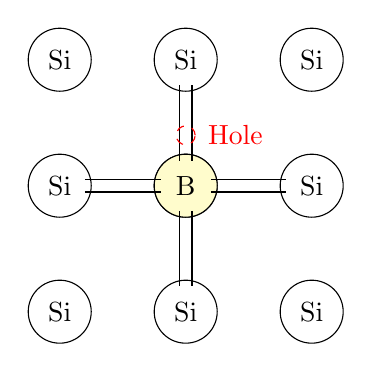
\begin{tikzpicture}[scale=0.8]
    \foreach \x in {0,2,4}
    \foreach \y in {0,2,4}
        \node [draw, circle, minimum size=0.8cm] at (\x,\y) {Si};
    
    \node [draw, circle, minimum size=0.8cm, fill=yellow!20] at (2,2) {B};
    
    % Bonds
    \draw (0.4, 2.1) -- (1.6, 2.1); \draw (0.4, 1.9) -- (1.6, 1.9); % Left
    \draw (2.4, 2.1) -- (3.6, 2.1); \draw (2.4, 1.9) -- (3.6, 1.9); % Right
    \draw (2.1, 2.4) -- (2.1, 3.6); \draw (1.9, 2.4) -- (1.9, 3.6); % Top
    \draw (2.1, 1.6) -- (2.1, 0.4); \draw (1.9, 1.6) -- (1.9, 0.4); % Bottom
    
    % Hole
    \draw [red, dashed] (2, 2.8) circle (0.15);
    \node [red, right] at (2.2, 2.8) {Hole};
\end{tikzpicture}
\captionof{figure}{Boron atom in Silicon lattice creating a Hole}
\end{center}
\end{solutionbox}

\begin{mnemonicbox}
\mnemonic{Three Makes Positive: Three valence electrons make a Positive hole}
\end{mnemonicbox}

\questionmarks{2(a) OR}{3}{Enlist factors affecting Resistance and explain any one of them.}

\begin{solutionbox}
\textbf{Factors Affecting Resistance:}
\begin{enumerate}
    \item Length of conductor ($L$)
    \item Cross-sectional area ($A$)
    \item Material (Resistivity, $\rho$)
    \item Temperature ($T$)
\end{enumerate}

\textbf{Explanation of Temperature Effect:}
The resistance of most metallic conductors increases with temperature.
\[ R = R_0[1 + \alpha(T - T_0)] \]
Where:
\begin{itemize}
    \item $R$ = Resistance at temp $T$
    \item $R_0$ = Resistance at reference temp $T_0$
    \item $\alpha$ = Temperature coefficient of resistance
\end{itemize}
As temperature increases, atoms vibrate more, hindering electron flow, thus increasing resistance.
\end{solutionbox}

\begin{mnemonicbox}
\mnemonic{LAMT: Length, Area, Material, Temperature}
\end{mnemonicbox}

\questionmarks{2(b) OR}{4}{Define: 1. Valance band, 2. Conduction band, 3. Forbidden energy gap, 4. Free electron}

\begin{solutionbox}
\begin{itemize}
    \item \textbf{Valence band:} The energy band occupied by valence electrons that are bound to atoms.
    \item \textbf{Conduction band:} The higher energy band where electrons are free to move and conduct electricity.
    \item \textbf{Forbidden energy gap:} The energy difference between the valence band and conduction band where no electron states can exist.
    \item \textbf{Free electron:} An electron that has gained enough energy to jump from the valence band to the conduction band, leaving a hole behind.
\end{itemize}

\begin{center}
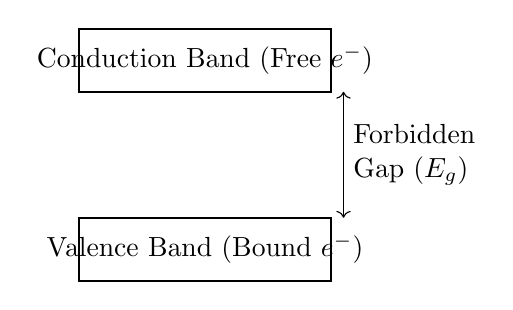
\begin{tikzpicture}[scale=0.8]
    \draw[thick] (0, 3) rectangle (4, 4);
    \node at (2, 3.5) {Conduction Band (Free $e^-$)};
    
    \draw[thick] (0, 0) rectangle (4, 1);
    \node at (2, 0.5) {Valence Band (Bound $e^-$)};
    
    \draw[<->] (4.2, 1) -- (4.2, 3);
    \node[right, align=left] at (4.2, 2) {Forbidden\\Gap ($E_g$)};
\end{tikzpicture}
\captionof{figure}{Energy Band Diagram}
\end{center}
\end{solutionbox}

\begin{mnemonicbox}
\mnemonic{Very Clearly Freedom Follows: Valence, Conduction, Forbidden gap, Free electrons}
\end{mnemonicbox}

\questionmarks{2(c) OR}{7}{Define Pentavalent material and give examples of it. Explain Formation of N-type material with the help of proper diagram.}

\begin{solutionbox}
\begin{itemize}
    \item \textbf{Pentavalent material:} Elements with 5 valence electrons in their outermost shell.
    \item \textbf{Examples:} Phosphorus (P), Arsenic (As), Antimony (Sb).
\end{itemize}

\textbf{Formation of N-type Semiconductor:}
When a pure Silicon crystal is doped with a pentavalent impurity (like Phosphorus):
\begin{enumerate}
    \item \textbf{Bond formation:} 4 of the valence electrons of Phosphorus form covalent bonds with 4 neighboring Silicon atoms.
    \item \textbf{Free electron:} The 5th valence electron is left loosely bound and easily becomes free to move.
    \item \textbf{Charge Carriers:} Electrons are negatively charged carriers. Electrons become \textbf{Majority carriers}, while holes are \textbf{Minority carriers}.
\end{enumerate}

\begin{center}
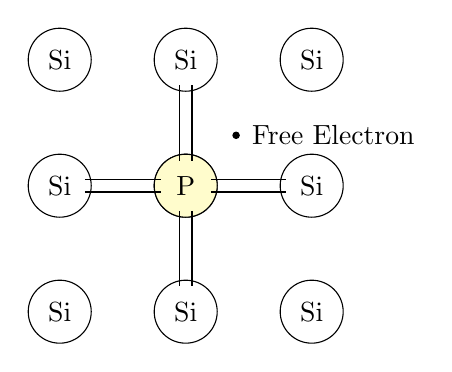
\begin{tikzpicture}[scale=0.8]
    \foreach \x in {0,2,4}
    \foreach \y in {0,2,4}
        \node [draw, circle, minimum size=0.8cm] at (\x,\y) {Si};
    
    \node [draw, circle, minimum size=0.8cm, fill=yellow!20] at (2,2) {P};
    
    % Bonds
    \draw (0.4, 2.1) -- (1.6, 2.1); \draw (0.4, 1.9) -- (1.6, 1.9); % Left
    \draw (2.4, 2.1) -- (3.6, 2.1); \draw (2.4, 1.9) -- (3.6, 1.9); % Right
    \draw (2.1, 2.4) -- (2.1, 3.6); \draw (1.9, 2.4) -- (1.9, 3.6); % Top
    \draw (2.1, 1.6) -- (2.1, 0.4); \draw (1.9, 1.6) -- (1.9, 0.4); % Bottom
    
    % Free Electron
    \draw [fill=black] (2.8, 2.8) circle (0.05);
    \node [right] at (2.9, 2.8) {Free Electron};
\end{tikzpicture}
\captionof{figure}{Phosphorus atom in Silicon lattice creating a Free Electron}
\end{center}
\end{solutionbox}

\begin{mnemonicbox}
\mnemonic{Five Makes Negative: Five valence electrons make a Negative carrier}
\end{mnemonicbox}

\questionmarks{3(a)}{3}{Define: 1. Depletion region, 2. Knee voltage, 3. Breakdown voltage in accordance of diode.}

\begin{solutionbox}
\begin{enumerate}
    \item \textbf{Depletion region:} The region near the P-N junction that is depleted of mobile charge carriers due to diffusion and recombination of electrons and holes. It contains only immobile ions.
    \item \textbf{Knee voltage ($V_k$):} The minimum forward voltage at which current starts increasing rapidly. (Approx. 0.7V for Si, 0.3V for Ge). Also called cut-in voltage.
    \item \textbf{Breakdown voltage ($V_{BR}$):} The reverse voltage at which the P-N junction breaks down and allows a large reverse current to flow, potentially damaging the diode.
\end{enumerate}
\end{solutionbox}

\begin{mnemonicbox}
\mnemonic{Depleted Knees Break: Depletion occurs, Knee begins conduction, Breakdown ends blocking}
\end{mnemonicbox}

\questionmarks{3(b)}{4}{Explain V-I characteristics of P-N junction diode with necessary graph.}

\begin{solutionbox}
The V-I characteristic shows the relationship between voltage across the diode and current flowing through it.

\begin{enumerate}
    \item \textbf{Forward Bias ($V > 0$):} Initially, current is small. Once voltage exceeds Knee voltage ($V_k \approx 0.7V$), current increases exponentially.
    \item \textbf{Reverse Bias ($V < 0$):} Only a very small leakage current (saturation current $I_s$) flows.
    \item \textbf{Breakdown:} If reverse voltage exceeds Breakdown voltage ($V_{BR}$), current increases sharply.
\end{enumerate}

\begin{center}
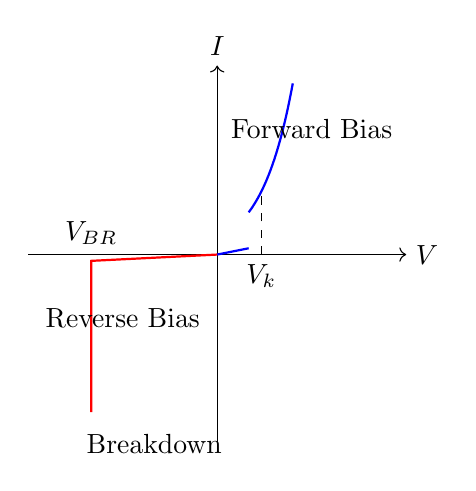
\begin{tikzpicture}[scale=0.8]
    \draw[->] (-3,0) -- (3,0) node[right] {$V$};
    \draw[->] (0,-3) -- (0,3) node[above] {$I$};
    
    % Forward
    \draw[blue, thick] (0,0) -- (0.5,0.1) plot[domain=0.5:1.2] (\x, {exp(2*(\x-0.7))});
    \node at (1.5, 2) {Forward Bias};
    \draw[dashed] (0.7,0) -- (0.7,1);
    \node[below] at (0.7,0) {$V_k$};
    
    % Reverse
    \draw[red, thick] (0,0) -- (-2, -0.1) -- (-2, -2.5);
    \node at (-1.5, -1) {Reverse Bias};
    \node[above] at (-2,0) {$V_{BR}$};
    \node at (-1, -3) {Breakdown};
\end{tikzpicture}
\captionof{figure}{V-I Characteristics of PN Junction Diode}
\end{center}
\end{solutionbox}

\begin{mnemonicbox}
\mnemonic{Forward Flows, Reverse Restricts, Breakdown Bursts}
\end{mnemonicbox}

\questionmarks{3(c)}{7}{Draw characteristic of Varactor diode. Explain working of Varactor diode with diagram and write its application.}

\begin{solutionbox}
\textbf{Working of Varactor Diode:}
A Varactor (Variable Capacitor) diode works on the principle that the depletion region acts as a dielectric between the P and N conductive regions (acting as plates).
\begin{itemize}
    \item It acts as a voltage-dependent capacitor.
    \item Operated in \textbf{Reverse Bias}.
    \item As reverse voltage ($V_R$) increases, depletion width ($W$) increases. Since $C \propto 1/W$, capacitance \textbf{decreases}.
    \item Relation: $C = \frac{K}{\sqrt{V_R}}$
\end{itemize}

\begin{center}
\begin{tabular}{cc}
\begin{circuitikz}[scale=0.8]
    \draw (0,0) to[vC, l=Varactor] (2,0);
\end{circuitikz} &
\begin{tikzpicture}[scale=0.8]
    \draw[->] (0,0) -- (4,0) node[right] {$V_R$ (Reverse V)};
    \draw[->] (0,0) -- (0,3) node[above] {$C$ (Capacitance)};
    \draw[blue, thick] plot[domain=0.2:3.5] (\x, {2.5/sqrt(\x)});
\end{tikzpicture} \\
Symbol & Characteristics ($C$ vs $V_R$)
\end{tabular}
\end{center}

\textbf{Applications:}
\begin{itemize}
    \item Voltage Controlled Oscillators (VCOs)
    \item Frequency Modulation (FM) transmitters
    \item Automatic Frequency Control (AFC) in radios
    \item TV tuning circuits
\end{itemize}
\end{solutionbox}

\begin{mnemonicbox}
\mnemonic{Capacitance Varies Reversely: Capacitance Varies with Reverse voltage}
\end{mnemonicbox}

\questionmarks{3(a) OR}{3}{Write application of following diode: 1. Varactor diode, 2. Photo diode, 3. Light Emitting Diode}

\begin{solutionbox}
\begin{tabulary}{\linewidth}{|L|L|}
\hline
\textbf{Diode Type} & \textbf{Applications} \\ \hline
\textbf{Varactor Diode} & Tuning circuits, VCOs, Frequency Modulators. \\ \hline
\textbf{Photo Diode} & Light detectors, Solar cells, Optical communication receivers, Smoke detectors. \\ \hline
\textbf{LED} & Indicators, Digital displays (7-segment), Traffic lights, Lighting, Optical communication transmitters. \\ \hline
\end{tabulary}
\end{solutionbox}

\begin{mnemonicbox}
\mnemonic{Vary Photo Emit: Varactor varies frequency, Photo detects light, LED emits light}
\end{mnemonicbox}

\questionmarks{3(b) OR}{4}{Explain working of P-N junction diode in forward bias and reverse bias.}

\begin{solutionbox}
\begin{enumerate}
    \item \textbf{Forward Bias:} P-terminal connected to Positive, N-terminal to Negative.
    \begin{itemize}
        \item Holes from P and electrons from N are pushed towards the junction.
        \item Depletion width decreases.
        \item Low resistance path; current flows easily.
    \end{itemize}
    \item \textbf{Reverse Bias:} P-terminal connected to Negative, N-terminal to Positive.
    \begin{itemize}
        \item Holes from P and electrons from N are pulled away from the junction.
        \item Depletion width increases.
        \item High resistance path; almost no current flows (except tiny leakage).
    \end{itemize}
\end{enumerate}

\begin{center}
\begin{tabular}{cc}
\begin{circuitikz}[scale=0.7]
    \draw (0,0) to[battery1, l=$V$] (0,2) -- (1,2)
    to[D*, l=Diode] (3,2) -- (3,0) -- (0,0);
    \node at (1.5,-0.5) {Forward Bias};
\end{circuitikz} &
\begin{circuitikz}[scale=0.7]
    \draw (0,0) to[battery1, l=$V$, invert] (0,2) -- (1,2)
    to[D*, l=Diode] (3,2) -- (3,0) -- (0,0);
    \node at (1.5,-0.5) {Reverse Bias};
\end{circuitikz}
\end{tabular}
\end{center}
\end{solutionbox}

\begin{mnemonicbox}
\mnemonic{Forward Flows, Reverse Resists}
\end{mnemonicbox}

\questionmarks{3(c) OR}{7}{Draw characteristic of Photo diode. Explain working of Photo diode with diagram and write its application.}

\begin{solutionbox}
\textbf{Working of Photo Diode:}
A Photo diode is a PN junction diode designed to operate in \textbf{Reverse Bias}. It has a transparent window to allow light to strike the junction.
\begin{itemize}
    \item When light (photons) strikes the depletion region, it generates electron-hole pairs.
    \item The reverse bias electric field sweeps these carriers across the junction, creating a current.
    \item This reverse current is proportional to the light intensity ($I_{light} \propto \Phi$).
\end{itemize}

\begin{center}
\begin{tabular}{cc}
\begin{circuitikz}[scale=0.8]
    \draw (0,0) to[photodiode, l=PD] (2,0);
\end{circuitikz} &
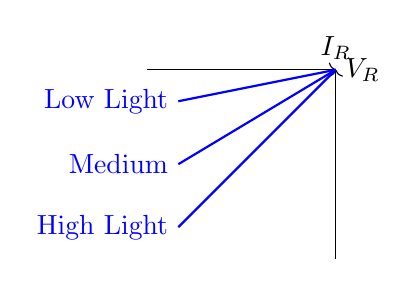
\begin{tikzpicture}[scale=0.8]
    \draw[->] (-3,0) -- (0,0) node[right] {$V_R$};
    \draw[->] (0,-3) -- (0,0) node[above] {$I_R$};
    
    \draw[blue, thick] (0,0) -- (-2.5, -0.5) node[left] {Low Light};
    \draw[blue, thick] (0,0) -- (-2.5, -1.5) node[left] {Medium};
    \draw[blue, thick] (0,0) -- (-2.5, -2.5) node[left] {High Light};
\end{tikzpicture} \\
Symbol & Characteristics
\end{tabular}
\end{center}

\textbf{Applications:}
\begin{itemize}
    \item Light sensors (street lights)
    \item Optical fiber receivers
    \item Remote control receivers
    \item Security alarms
\end{itemize}
\end{solutionbox}

\begin{mnemonicbox}
\mnemonic{Light In, Current Out: Light intensity controls current output}
\end{mnemonicbox}

\questionmarks{4(a)}{3}{Explain working of Half wave rectifier with circuit diagram.}

\begin{solutionbox}
\textbf{Half Wave Rectifier:}
\begin{center}
\begin{tabular}{cc}
\begin{circuitikz}[scale=0.8]
    \draw (0,0) to[sV, l=$V_{in}$] (0,2) 
    to[D, l=D] (2,2) 
    to[R, l=$R_L$] (2,0) -- (0,0);
    \draw (2,2) -- (3,2) node[right] {$+$};
    \draw (2,0) -- (3,0) node[right] {$-$ $V_{out}$};
\end{circuitikz} &
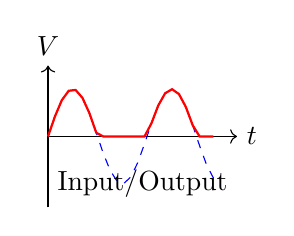
\begin{tikzpicture}[scale=0.6]
    \draw[->] (0,0) -- (4,0) node[right] {$t$};
    \draw[->] (0,-1.5) -- (0,1.5) node[above] {$V$};
    \draw[blue, dashed] plot[domain=0:3.5] (\x, {sin(\x r * 3)});
    \draw[red, thick] plot[domain=0:3.5] (\x, {max(0, sin(\x r * 3))});
    \node at (2, -1) {Input/Output};
\end{tikzpicture}
\end{tabular}
\captionof{figure}{Half Wave Rectifier Circuit and Waveform}
\end{center}

\begin{tabulary}{\linewidth}{|L|L|}
\hline
\textbf{Operation Phase} & \textbf{Description} \\ \hline
\textbf{Positive Half Cycle} & Diode is forward biased and conducts. Current flows through load. Output follows input. \\ \hline
\textbf{Negative Half Cycle} & Diode is reverse biased and blocks current. Output voltage is zero. \\ \hline
\end{tabulary}

\begin{itemize}
    \item \textbf{Output frequency:} $f_{out} = f_{in}$
    \item \textbf{Efficiency:} 40.6\%
    \item \textbf{Ripple factor:} 1.21
\end{itemize}
\end{solutionbox}

\begin{mnemonicbox}
\mnemonic{Half Passes Positive: Only positive half-cycle passes through}
\end{mnemonicbox}

\questionmarks{4(b)}{4}{Explain Zener diode as a voltage regulator.}

\begin{solutionbox}
\textbf{Zener Diode Voltage Regulator:}
\begin{center}
\begin{circuitikz}[scale=0.9]
    \draw (0,0) to[battery1, l=$V_{in}$] (0,3) to[R, l=$R_S$] (3,3) -- (5,3);
    \draw (3,3) to[zD*, l=$D_Z$] (3,0);
    \draw (5,3) to[R, l=$R_L$] (5,0);
    \draw (0,0) -- (5,0);
    \node at (5.5, 1.5) {$V_{out} = V_Z$};
\end{circuitikz}
\captionof{figure}{Zener Voltage Regulator}
\end{center}

\textbf{Working Principle:}
\begin{enumerate}
    \item The Zener diode is connected in parallel with the load in \textbf{reverse bias}.
    \item It operates in the breakdown region where voltage across it ($V_Z$) remains constant for a wide range of currents.
    \item \textbf{Line Regulation:} If input voltage $V_{in}$ increases, current through Zener increases, but voltage drop across $R_L$ remains constant at $V_Z$. Excess voltage drops across $R_S$.
    \item \textbf{Load Regulation:} If load current changes, Zener current adjusts to keep total current constant enough to maintain $V_{out} = V_Z$.
\end{enumerate}
\end{solutionbox}

\begin{mnemonicbox}
\mnemonic{Zener Zeros Voltage Variations}
\end{mnemonicbox}

\questionmarks{4(c)}{7}{Write need of Rectifier. Explain Bridge wave rectifier with circuit diagram and draw its input and output waveform.}

\begin{solutionbox}
\textbf{Need of Rectifier:}
\begin{itemize}
    \item To convert AC voltage (from mains) to DC voltage.
    \item Most electronic devices (TV, Computers, Mobiles) require DC power to operate.
\end{itemize}

\textbf{Bridge Wave Rectifier:}
\begin{center}
\begin{circuitikz}[scale=0.8]
    \draw (0,0) to[sV, l=$V_{in}$] (0,3);
    \draw (0,3) -- (2,3) -- (3,2);
    \draw (0,0) -- (2,0) -- (5,0) -- (5,2);
    
    % Bridge
    \draw (3,2) to[D*, l=$D_1$] (4,3);
    \draw (4,3) to[D*, l=$D_2$] (5,2);
    \draw (5,2) to[D*, l=$D_3$] (4,1);
    \draw (4,1) to[D*, l=$D_4$] (3,2);
    
    % Load
    \draw (4,3) -- (4,4) -- (7,4) to[R, l=$R_L$] (7,0) -- (5,0);
    \draw (4,1) to[short,-*] (4,1) -- (4,0); % Ground connection visually
    \node at (7.5, 2) {$V_{out}$};
\end{circuitikz}
\captionof{figure}{Bridge Rectifier Circuit}
\end{center}

\textbf{Waveforms:}
\begin{center}
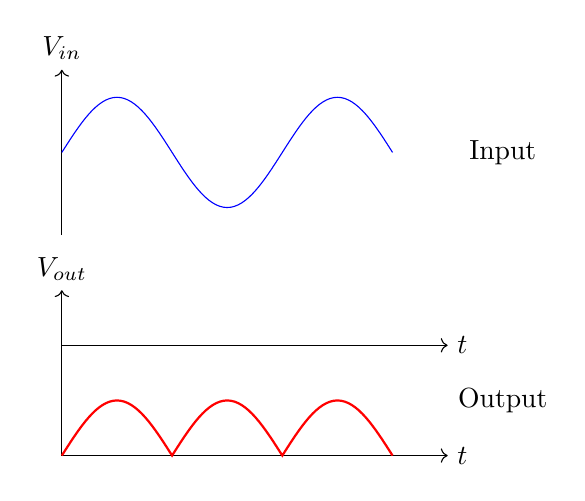
\begin{tikzpicture}[scale=0.7]
    \draw[->] (0,0) -- (7,0) node[right] {$t$};
    \draw[->] (0,2) -- (0,5) node[above] {$V_{in}$};
    \draw[blue] (0,3.5) sin (1,4.5) cos (2,3.5) sin (3,2.5) cos (4,3.5) sin (5,4.5) cos (6,3.5);
    \node at (8, 3.5) {Input};
    
    \draw[->] (0,-2) -- (7,-2) node[right] {$t$};
    \draw[->] (0,-2) -- (0,1) node[above] {$V_{out}$};
    \draw[red, thick] (0,-2) sin (1,-1) cos (2,-2) sin (3,-1) cos (4,-2) sin (5,-1) cos (6,-2);
    \node at (8, -1) {Output};
\end{tikzpicture}
\captionof{figure}{Input and Output Waveforms}
\end{center}

\begin{itemize}
    \item \textbf{Positive Half Cycle:} $D_1$ and $D_3$ conduct.
    \item \textbf{Negative Half Cycle:} $D_2$ and $D_4$ conduct.
    \item Current flows through $R_L$ in the same direction in both half cycles.
    \item Efficiency: 81.2\%
\end{itemize}
\end{solutionbox}

\begin{mnemonicbox}
\mnemonic{Bridge Both Better: Bridge rectifier uses both half cycles}
\end{mnemonicbox}

\questionmarks{4(a) OR}{3}{Explain working of Shunt capacitor filter.}

\begin{solutionbox}
\textbf{Shunt Capacitor Filter:}
\begin{center}
\begin{circuitikz}[scale=0.8]
    \draw (0,0) to[sV, l=Rectifier] (0,2) -- (2,2);
    \draw (2,2) to[C, l=$C$] (2,0);
    \draw (2,2) -- (4,2) to[R, l=$R_L$] (4,0) -- (0,0);
    \draw (2,0) -- (0,0);
\end{circuitikz}
\end{center}
\begin{itemize}
    \item \textbf{Charging:} When rectifier voltage increases, Capacitor charges to peak voltage $V_m$.
    \item \textbf{Discharging:} When rectifier voltage falls, Capacitor discharges through $R_L$, maintaining voltage.
    \item \textbf{Result:} Smoother DC output with reduced ripple.
\end{itemize}
\end{solutionbox}

\begin{mnemonicbox}
\mnemonic{Capacitor Catches Peaks: Capacitor stores peak voltage}
\end{mnemonicbox}

\questionmarks{4(b) OR}{4}{Compare Center tap full wave rectifier and Bridge wave rectifier}

\begin{solutionbox}
\begin{tabulary}{\linewidth}{|L|L|L|}
\hline
\textbf{Parameter} & \textbf{Center Tap FW Rectifier} & \textbf{Bridge Rectifier} \\ \hline
\textbf{No. of Diodes} & 2 & 4 \\ \hline
\textbf{Transformer} & Center-tapped required (Bulky, costly) & Simple transformer (Smaller, cheaper) \\ \hline
\textbf{PIV Rating} & $2V_m$ & $V_m$ \\ \hline
\textbf{Efficiency} & 81.2\% & 81.2\% \\ \hline
\textbf{Cost} & Higher (due to transformer) & Lower \\ \hline
\end{tabulary}
\end{solutionbox}

\begin{mnemonicbox}
\mnemonic{Center Taps Transformer, Bridge Bypasses Tapping}
\end{mnemonicbox}

\questionmarks{4(c) OR}{7}{Write need of Filter circuit in rectifier. Explain $\pi$ filter with circuit diagram and draw its input and output waveform.}

\begin{solutionbox}
\textbf{Need of Filter:}
To remove AC components (ripple) from the rectifier output and provide a steady/smooth DC voltage suitable for electronic circuits.

\textbf{$\pi$ Filter (CLC Filter):}
\begin{center}
\begin{circuitikz}[scale=0.8]
    \draw (0,0) to[sV, l=In] (0,2) -- (1,2);
    \draw (1,2) to[C, l=$C_1$] (1,0);
    \draw (1,2) to[L, l=$L$] (3,2);
    \draw (3,2) to[C, l=$C_2$] (3,0);
    \draw (3,2) -- (4,2) to[R, l=$R_L$] (4,0) -- (0,0);
    \draw (1,0) -- (0,0); % Ground
    \draw (3,0) -- (1,0);
\end{circuitikz}
\captionof{figure}{$\pi$ (Pi) Filter Circuit}
\end{center}

\begin{itemize}
    \item \textbf{$C_1$}: Bypasses most AC ripple to ground.
    \item \textbf{$L$}: Blocks remaining AC (high impedance to AC) but passes DC.
    \item \textbf{$C_2$}: Filters any residual ripple.
\end{itemize}

\textbf{Waveforms:}
\begin{center}
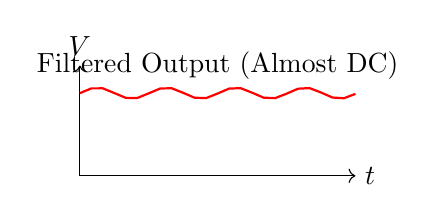
\begin{tikzpicture}[scale=0.7]
    \draw[->] (0,0) -- (5,0) node[right] {$t$};
    \draw[->] (0,0) -- (0,2) node[above] {$V$};
    \draw[red, thick] plot[domain=0:5] (\x, {1.5 + 0.1*sin(\x r * 5)});
    \node at (2.5, 2) {Filtered Output (Almost DC)};
\end{tikzpicture}
\end{center}
\end{solutionbox}

\begin{mnemonicbox}
\mnemonic{Capacitor-Inductor-Capacitor Perfectly Irons}
\end{mnemonicbox}

\questionmarks{5(a)}{3}{Explain Working of PNP Transistor with the necessary diagram.}

\begin{solutionbox}
\textbf{PNP Transistor:}
A PNP transistor consists of a thin N-type base sandwiched between two P-type regions (Emitter and Collector).

\begin{center}
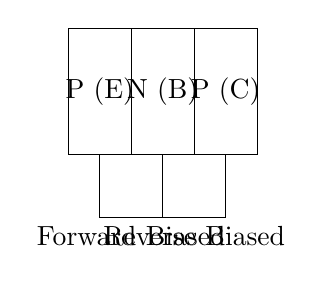
\begin{tikzpicture}[scale=0.8]
    \draw (0,0) rectangle (3,2);
    \draw (1,0) -- (1,2);
    \draw (2,0) -- (2,2);
    \node at (0.5,1) {P (E)};
    \node at (1.5,1) {N (B)};
    \node at (2.5,1) {P (C)};
    
    % Biasing
    \draw (0.5,0) -- (0.5,-1) -- (1.5,-1);
    \draw (1.5,0) -- (1.5,-1);
    \node at (1,-1.3) {Forward Biased};
    
    \draw (2.5,0) -- (2.5,-1) -- (1.5,-1);
    \node at (2,-1.3) {Reverse Biased};
\end{tikzpicture}
\end{center}

\begin{itemize}
    \item \textbf{Emitter-Base Junction:} Forward Biased. Holes move from Emitter to Base.
    \item \textbf{Collector-Base Junction:} Reverse Biased. Holes that cross the Base are collected by the Collector.
    \item Majority carriers: Holes. Current flow is from Emitter to Collector.
\end{itemize}
\end{solutionbox}

\begin{mnemonicbox}
\mnemonic{Positive-Negative-Positive}
\end{mnemonicbox}

\questionmarks{5(b)}{4}{Explain working of N-channel JFET with diagram.}

\begin{solutionbox}
\textbf{N-channel JFET:}
\begin{center}
\begin{circuitikz}[scale=0.8]
    \draw (0,0) node[njfet] (Q) {};
    \node[right] at (Q.D) {Drain};
    \node[right] at (Q.S) {Source};
    \node[left] at (Q.G) {Gate};
    
    % Channel illustration
    \draw (2, -1) rectangle (3, 1); \node at (2.5,0) {N-Ch};
    \draw[fill=gray] (1.8, 0) rectangle (2, 0.5); \node[left] at (1.8, 0.25) {P (Gate)};
    \draw[fill=gray] (3, 0) rectangle (3.2, 0.5); \node[right] at (3.2, 0.25) {P (Gate)};
\end{circuitikz}
\end{center}

\textbf{Working:}
\begin{itemize}
    \item Current flows from Drain to Source through the N-channel.
    \item A reverse voltage is applied to the Gate ($V_{GS} < 0$).
    \item Increasing negative gate voltage widens the depletion region, narrowing the channel.
    \item This increases resistance and reduces Drain current ($I_D$). Hence, it's a Voltage Controlled Device.
\end{itemize}
\end{solutionbox}

\begin{mnemonicbox}
\mnemonic{Negative Channel Junction Effect}
\end{mnemonicbox}

\questionmarks{5(c)}{7}{Compare BJT and JFET}

\begin{solutionbox}
\begin{tabulary}{\linewidth}{|L|L|L|}
\hline
\textbf{Parameter} & \textbf{BJT} & \textbf{JFET} \\ \hline
\textbf{Type} & Bipolar (Electrons \& Holes) & Unipolar (Majority carriers only) \\ \hline
\textbf{Control} & Current Controlled Device ($I_B$ controls $I_C$) & Voltage Controlled Device ($V_{GS}$ controls $I_D$) \\ \hline
\textbf{Input Impedance} & Low ($k\Omega$ range) & Very High ($M\Omega$ range) \\ \hline
\textbf{Noise} & Higher noise level & Low noise \\ \hline
\textbf{Temp Stability} & Lower & Higher \\ \hline
\textbf{Size} & Larger & Smaller (easier to fabricate in ICs) \\ \hline
\end{tabulary}
\end{solutionbox}

\begin{mnemonicbox}
\mnemonic{Current Bipolar Low, Voltage Unipolar High}
\end{mnemonicbox}

\questionmarks{5(a) OR}{3}{Enlist methods to dispose E-waste and explain any one method of them.}

\begin{solutionbox}
\textbf{Methods:}
\begin{enumerate}
    \item Recycling
    \item Reuse
    \item Incineration
    \item Landfilling
    \item Take-back systems
\end{enumerate}

\textbf{Recycling:}
Involves dismantling electronic devices and separating materials like plastic, glass, and metals (Gold, Copper, etc.). These recovered materials are processed and used to manufacture new products. It significantly reduces environmental pollution and conserves natural resources.
\end{solutionbox}

\begin{mnemonicbox}
\mnemonic{RRIL-T: Recycling, Reuse, Incineration, Landfill, Take-back}
\end{mnemonicbox}

\questionmarks{5(b) OR}{4}{Compare PNP and NPN Transistor.}

\begin{solutionbox}
\begin{tabulary}{\linewidth}{|L|L|L|}
\hline
\textbf{Parameter} & \textbf{PNP} & \textbf{NPN} \\ \hline
\textbf{Structure} & P-N-P Layers & N-P-N Layers \\ \hline
\textbf{Majority Carriers} & Holes & Electrons \\ \hline
\textbf{Collector Current} & Due to flows of holes & Due to flow of electrons \\ \hline
\textbf{Biasing} & Base is negative w.r.t Emitter & Base is positive w.r.t Emitter \\ \hline
\textbf{Speed} & Slower (hole mobility is low) & Faster (electron mobility is high) \\ \hline
\textbf{Preferred Usage} & Less common & Most common \\ \hline
\end{tabulary}
\end{solutionbox}

\begin{mnemonicbox}
\mnemonic{Positive-Negative-Positive (Holes), Negative-Positive-Negative (Electrons)}
\end{mnemonicbox}

\questionmarks{5(c) OR}{7}{Draw and explain Input and Output Characteristics of CE configuration.}

\begin{solutionbox}
\textbf{1. Input Characteristics ($I_B$ vs $V_{BE}$):}
It is a graph of Base current against Base-Emitter voltage at constant $V_{CE}$. It resembles a forward-biased diode curve.
\begin{center}
\begin{tikzpicture}[scale=0.7]
    \draw[->] (0,0) -- (4,0) node[right] {$V_{BE}$};
    \draw[->] (0,0) -- (0,3) node[above] {$I_B$};
    \draw[blue, thick] (0.7,0) .. controls (1,0.5) and (1.2,2) .. (1.5,3);
    \node at (2,1) {$V_{CE} > 0$};
\end{tikzpicture}
\end{center}

\textbf{2. Output Characteristics ($I_C$ vs $V_{CE}$):}
Graph of Collector current against Collector-Emitter voltage at constant $I_B$.
\begin{itemize}
    \item \textbf{Cut-off Region:} Both junctions reverse biased. $I_C \approx 0$.
    \item \textbf{Active Region:} JE forward, JC reverse biased. $I_C = \beta I_B$. Used for amplification.
    \item \textbf{Saturation Region:} Both junctions forward biased. $V_{CE}$ is very low. Used for switching (ON).
\end{itemize}

\begin{center}
\begin{tikzpicture}[scale=0.7]
    \draw[->] (0,0) -- (4,0) node[right] {$V_{CE}$};
    \draw[->] (0,0) -- (0,4) node[above] {$I_C$};
    \draw (0,0) -- (0.5, 3) -- (4, 3.2) node[right] {$I_{B3}$};
    \draw (0,0) -- (0.5, 2) -- (4, 2.2) node[right] {$I_{B2}$};
    \draw (0,0) -- (0.5, 1) -- (4, 1.2) node[right] {$I_{B1}$};
    
    \node[draw, dashed, fit={(0,0) (0.5,3.5)}] (sat) {}; \node[above] at (sat.north) {Sat};
    \node[draw, dashed, fit={(0,0) (4,0.5)}] (cut) {}; \node[right] at (cut.east) {Cut-off};
    \node at (2,2.5) {Active};
\end{tikzpicture}
\end{center}
\end{solutionbox}

\begin{mnemonicbox}
\mnemonic{Input Shows Voltage Effects, Output Shows Current Control}
\end{mnemonicbox}

\end{document}
